\documentclass[a4paper,11pt]{report}
\usepackage[T1]{fontenc}
\usepackage[utf8]{inputenc}
\usepackage[francais]{babel}
\usepackage[babel=true,kerning=true]{microtype}
\usepackage[usenames,dvipsnames,svgnames,table]{xcolor}
\usepackage[colorlinks,linkcolor={blue!30!black},citecolor={blue!50!black},urlcolor={blue!80!black}]{hyperref}
\usepackage{amsmath,amsfonts,amssymb,array,graphicx,caption,lmodern,subcaption,tikz,url,xspace,wrapfig}
\usepackage{textcomp,rotating,epic,pdfpages,listings,diagbox,multirow,float}
\usepackage{pgfplots}
\pgfplotsset{width=7cm,compat=1.8}

\usepackage[top=25mm,bottom=25mm,left=25mm,right=25mm]{geometry}
\parskip=6pt % Espacement vertical entre les paragraphes

\begin{document}
\pagenumbering{gobble}  % Pas de numérotation
\begin{titlepage}
    \vspace*{50px}
    
\includegraphics[height=80px]{Images/logo_phelma.pdf}
    \vspace*{-80px}
\begin{flushright}
%     \vspace*{60px}
    
\includegraphics[height=65px]{Images/CIME.jpg}
\end{flushright}

\vspace*{2cm}

\begin{center}
\rule{\linewidth}{0.5mm}\\[0.4cm]
{\huge{\bfseries Compte Rendu}\\[0.4cm]
\textsc{TP Simulation électronique}\\[0.4cm]}
\rule{\linewidth}{0.5mm}\\[0.5cm]

\LARGE{\textsc{Nicolas Paillet, Félix Piédallu \& Giulia Rizzo}}\\[0.7cm]
\large{\textsc{2015-2016}}\\[2cm]

\Large{~}\\[1cm]
% 
\includegraphics[width=0.4\textwidth]{Images/CIME.jpg}\\[1cm]
%
 \large{Encadrant : Marco Pala}\\[2cm]
%

\end{center}
\end{titlepage}

\tableofcontents        % Table des matières avec liens, générée automatiquement.
\newpage
\pagenumbering{arabic}  % Numérotation de retour !

\chapter*{Introduction} \addcontentsline{toc}{chapter}{Introduction}
Nous avons vu lors de notre cours d'Optique Non Linéaire que certains cristaux ne se comportent pas de manière isotrope et linéaire lorsqu'on leur impose un rayonnement Laser.

Le but de ce TP est donc d'étudier le comportement d'un cristal de RbTiOPO$_4$ (RTP).

Dans une première partie nous avons utilisé un laser He:Ne de longueur d'onde $\lambda = 632.8nm$ pour faire apparaître le caractère anisotrope du cristal qui se traduit par la séparation des deux composantes de polarisation de la lumière par le cristal (Chapitres \ref{OCLTheorie} et \ref{OCLExp}).

La seconde partie portera sur le calculs des conditions de Génération de seconde harmonique (SHG) (Chapitre \ref{ONLTheorie}) puis l'utilisation d'un laser NdYAG ($\lambda = 1064nm$, invisible) qui nous a permis d'observer le caractère non linéaire du cristal par un doublage de fréquence de l'onde incidente de l'infrarouge vers la lumière visible (Chapitre \ref{ONLExp}).

\chapter{Optique Cristalline Linéaire (Théorie)} \label{OCLTheorie}
\section{Surface des indices}
\subsection{Introduction: la susceptibilité électrique}
Dans un milieu quelconque, la susceptibilité électrique linéaire $\chi^{(1)}$ n'est pas forcément un scalaire. On peut de manière générale le représenter par un tenseur de rang 2 (i.e une matrice), dépendant de la direction de propagation de l'onde incidente.

Ce tenseur est diagonalisable dans le repère diélectrique, qui peut être totalement différent du repère cristallographique. On l'écrit alors sous cette forme:
\[\chi^{(1)} = 
\left( \begin{matrix}
\chi^{(1)}_{xx}   & 0                 & 0 \\
0                 & \chi^{(1)}_{yy}   & 0 \\
0                 & 0                 & \chi^{(1)}_{zz}
\end{matrix}\right) \]

La complexité de cette matrice est dépendante des symétries du cristal considéré: Plus il est de haute symétrie, plus on aura de valeurs propres égales:\\
Un milieu isotrope aura ses trois valeurs propres égales, un milieu biaxe aura $\chi^{(1)}_{xx} = \chi^{(1)}_{yy} \neq \chi^{(1)}_{zz}$, et un milieu biaxe aura ses trois valeurs propres différentes.

Le cristal de RbTiOPO$_4$ (RTP) cristallise dans un système orthorhombique, et admet une symétrie d'orientation $mm2$. Il est peu symétrique, il est alors de classe optique biaxe.

De plus il est orthorhombique, le repère cristallographique sera alors parallèle au repère diélectrique.
\vspace*{5mm}

\subsection{L'indice de réfraction}
L'indice de réfraction du milieu est directement lié à la susceptibilité électrique: dans un milieu isotrope, on a $n = \sqrt{1+\chi^{(1)}}$.

Dans un milieu anisotrope, cela devient un peu plus complexe. On va commencer par définir les indices de réfraction principaux:
\[  n_i = \sqrt{1+\chi^{(1)}_{ii}} \text{, avec } i=\{x, y, z\} \]

On peut alors écrire l'équation de Fresnel, tirée des équations de Maxwell:
\[
    \dfrac{\sin^2(\theta)\cdot\cos^2(\phi)}{\dfrac{1}{n^2(\theta, \phi, \lambda)} - \dfrac{1}{n^2_x(\lambda)}}
 +  \dfrac{\sin^2(\theta)\cdot\sin^2(\phi)}{\dfrac{1}{n^2(\theta, \phi, \lambda)} - \dfrac{1}{n^2_y(\lambda)}}
 +  \dfrac{\cos^2(\theta)                 }{\dfrac{1}{n^2(\theta, \phi, \lambda)} - \dfrac{1}{n^2_z(\lambda)}}
    = 0
\]

Cette équation quadratique en $n^2$ admet deux solutions:
\[
    n^+(\theta, \phi, \lambda) = \dfrac{\sqrt 2}{\sqrt{-B-B\sqrt{B^2-4C}}}
    \text{ et }
    n^-(\theta, \phi, \lambda) = \dfrac{\sqrt 2}{\sqrt{-B+B\sqrt{B^2-4C}}}
\]

avec: 
\[ B =  -sin^2(\theta) cos^2(\phi)  \left[\dfrac{1}{n^2_y(\lambda)} + \dfrac{1}{n^2_z(\lambda)}\right]
        -sin^2(\theta) sin^2(\phi)  \left[\dfrac{1}{n^2_x(\lambda)} + \dfrac{1}{n^2_z(\lambda)}\right]
        -cos^2(\theta)              \left[\dfrac{1}{n^2_x(\lambda)} + \dfrac{1}{n^2_y(\lambda)}\right]
\]

et:
\[ C =  \dfrac{sin^2(\theta) cos^2(\phi)}{n^2_y(\lambda)n^2_z(\lambda)}
     +  \dfrac{sin^2(\theta) sin^2(\phi)}{n^2_x(\lambda)n^2_z(\lambda)}
     +  \dfrac{cos^2(\theta)            }{n^2_x(\lambda)n^2_y(\lambda)}
\]

\subsection{Surface des indices}
Cela définit alors deux nappes intérieure et extérieure, car $n^+ \geq n^-$ est toujours vérifié.

Dans le cas d'un milieu biaxe, les surfaces d'indice ont la forme visible en fig. \ref{surf_indices}:

\begin{figure}[h]
    \begin{center}
        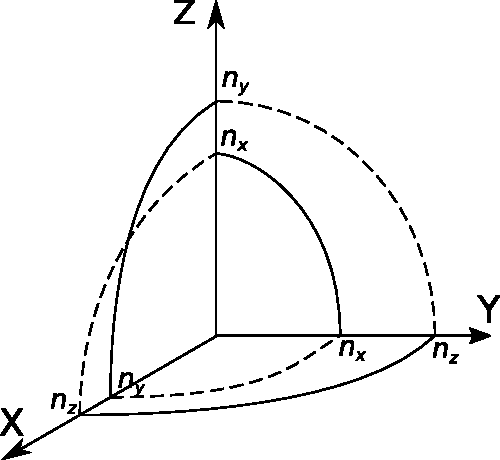
\includegraphics[width=0.4\textwidth]{Images/surface_indices}
        \caption{Surface des indices d'un cristal biaxe}
        \label{surf_indices}
    \end{center}
\end{figure}

\paragraph{L'équation de ces nappes} sur le plan $(\vec x, \vec z)$ est de la forme:
\[  \frac{1}{n^2_\text{ellipse}} = \frac{\cos^2(\theta)}{n^2_x} + \frac{\sin^2(\theta)}{n^2_z} \]
\[  n^2_\text{cercle} = n_y \]

La direction de propagation de l'onde électromagnétique est déterminée par l'intersection des nappes $n^+$ et $n^-$, c'est-à-dire par la solution double de l'équation de Fresnel:
\[  n(\theta, \phi, \lambda) = \dfrac{\sqrt 2}{\sqrt{-B}} \]

L'angle de propagation $V_z$ est alors défini par:
\[ \sin^2(V_z) = \frac{n_y^{-2}-n_x^{-2}}{n_z^{-2}-n_x^{-2}} \]


\section{Aparallélisme des champs}
Une susceptibilité électrique non scalaire implique alors que la polarisation du milieu ne soit pas parallèle au champ électrique:
\[\vec{P} = \varepsilon_0 \chi^{(1)} \cdot\vec{E}\]

et: 
\[\vec{D} = \varepsilon_0 \vec{E} + \vec{P}
          = \varepsilon_0 (1+\chi^{(1)}) \cdot\vec{E}
          = \varepsilon_0 \varepsilon_r^{(1)} \vec{E}\]

Enfin, on a:
\begin{itemize}
    \item $\vec{\pi} \perp \vec{E}$
    \item $\vec{k}   \perp \vec{D}$
    \item $\vec{\pi} = \frac{1}{\mu_0} \vec{E}\wedge \vec{B}$
\end{itemize}

\begin{figure}[h]
    \begin{center}
        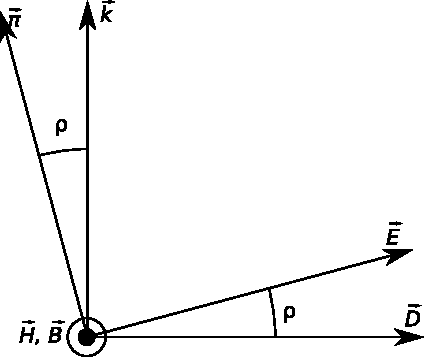
\includegraphics[width=0.4\textwidth]{Images/vecteurs.pdf}
        \caption{Vecteurs caractéristiques de l'onde}
        \label{vecteurs}
    \end{center}
\end{figure}


Il faut garder en tête que l'on observe physiquement $\vec{\pi}$ (la direction de propagation de l'énergie lumineuse, donc celle du rayon observable) et $\vec{E}$, et PAS $\vec{k}$ (la direction de l'onde électromagnétique) ni $\vec{D}$.

\section{Séparation des polarisations avec un cristal parallélépipédique}
Dans tout milieu anisotrope, une onde est en fait la somme de deux composantes $\vec{E}^+(\theta,\phi)$ et $\vec{E}^-(\theta,\phi)$, associées aux deux solutions de l'équation de Fresnel. Elles sont polarisées chacune rectilignement.

Dans les plans principaux, les deux polarisations sont orthogonales entre elles et:
\begin{itemize}
    \item L'onde associée à la nappe circulaire ($\vec{E}_{c}$) est polarisée orthogonalement au plan
    \item L'onde associée à la nappe ellipsoïdale ($\vec{E}_{e}$) est polarisée tangentiellement à l'ellipse.
\end{itemize}

\newpage
De plus à l'interface entre un milieu isotrope (l'air) et un milieu anisotrope (notre cristal RTP), il y a une variation d'indice optique anisotrope:
\begin{itemize}
    \item $\vec{k}$ et $\vec{D}$ ne varient pas: l'onde conserve la même direction de propagation
    \item $\vec{\pi}$ et $\vec{E}$ dévient: l'énergie lumineuse (le rayon) change de direction de propagation.\newline
\end{itemize}

Considérant que la propagation de l'énergie lumineuse ($\vec{\pi}$) est toujours orthogonale à la nappe d'indice:
\begin{itemize}
    \item $\vec{\pi}_{cercle}$ est parallèle à $\vec{k}_{cercle}$ et l'onde se propage sans changer de direction
    \item $\vec{\pi}_{ellipse}$ est dévié par rapport à $\vec{k}_{ellipse}$ et l'onde change de direction.
\end{itemize}

On a donc pu séparer les deux rayons comme on peut le constater sur la figure \ref{cristalparallelepipede}.

\begin{figure}[h]
    \begin{center}
        \begin{tikzpicture}
        \draw (4,0)--(8,0)--(8,2.5)--(4,2.5)--cycle;
        \draw (2,1)--(4,1)node[midway]{>};
        \draw (4,1)--(8,1)node[midway, below]{$\vec{\pi}_{cercle}$};
        \draw (8,1)--(10,1)node[midway]{>};
        \draw (4,1)--(8,2)node[midway, sloped, above]{$\vec{\pi}_{ellipse}$};
        \draw (8,2)--(10,2)node[midway]{>};
        \draw [-](6,1) arc(0:30:0.95) ;
        \draw (6.2,1.3)node{$\rho$};
        \draw [<->](10.2,1)--(10.2,2)node[midway, right]{d};
        \end{tikzpicture}
        \caption{Propagation des rayons dans le cristal parallélépipédique}
        \label{cristalparallelepipede}
    \end{center}
\end{figure}

En sortie du cristal, on a le même phénomène qu'en entrée: les deux faisceaux se retrouvent parallèles, mais séparés par une distance $\delta_z$.

Or l'angle $\rho$ est très faible habituellement, $\delta_z$ aussi. Cela ne nous permet pas d'effectuer une mesure précise.
\section{Séparation des polarisations avec un cristal cylindrique}
Une autre méthode est alors d'utiliser un cristal cylindrique.

\begin{figure}[h]
    \begin{center}
        \begin{tikzpicture}
        \draw (6,1) circle(2);
        \draw (2,1)--(4,1)node[midway]{>};
        \draw (4,1)--(8,1)node[midway, below]{$\vec{\pi}_{cercle}$};
        \draw (8,1)--(12,1)node[near end]{>};
        \draw (4,1)--(7.74,2)node[midway, sloped, above]{$\vec{\pi}_{ellipse}$};
        \draw (7.74,2)--(12,-2)node[near end, sloped]{>};
        \draw [-](6,1) arc(0:30:0.95); \draw (6.2,1.3)node{$\rho$};
        \draw [-](10,1) arc(0:-54:0.95); \draw (10.3,0.5)node{$\rho_{ext}$};
        \draw [<->](12.2,-2)--(12.2,1)node[midway, right]{d};
        \end{tikzpicture}
        \caption{Propagation des rayons dans le cristal cylindrique}
        \label{cristalcylindrique}
    \end{center}
\end{figure}

Comme $\rho_{ext}$ est assez grand, la mesure peut être très précise ; elle peut être améliorée en éloignant le capteur du cristal.

C'est cette configuration que nous avons utilisé dans la suite du TP.

De simples calculs géométriques prenant en compte notamment la distance entre le cristal et le capteur optique nous permettent de retrouver $\rho$ en fonction de la distance (linéaire) entre les deux faisceaux.

\chapter{Optique Cristalline Linéaire (Expérience)} \label{OCLExp}
\section{Mise en place de l'expérience}
Comme toute expérience d'optique, pour avoir un faisceau horizontal et tous les éléments optiques alignés correctement, on utilise une paire de miroirs entre le laser source He:Ne et le cristal: 

Le premier miroir permet d'amener le faisceau depuis la hauteur du laser, vers la même hauteur que le cristal. Le second miroir permet alors, sans modifier la hauteur du faisceau, d'ajuster uniquement sa direction pour qu'il soit horizontal.

On règle donc d'abord le premier miroir puis le second, plusieurs fois pour "converger" vers une configuration précise.

\begin{figure}[h]
    \begin{center}
        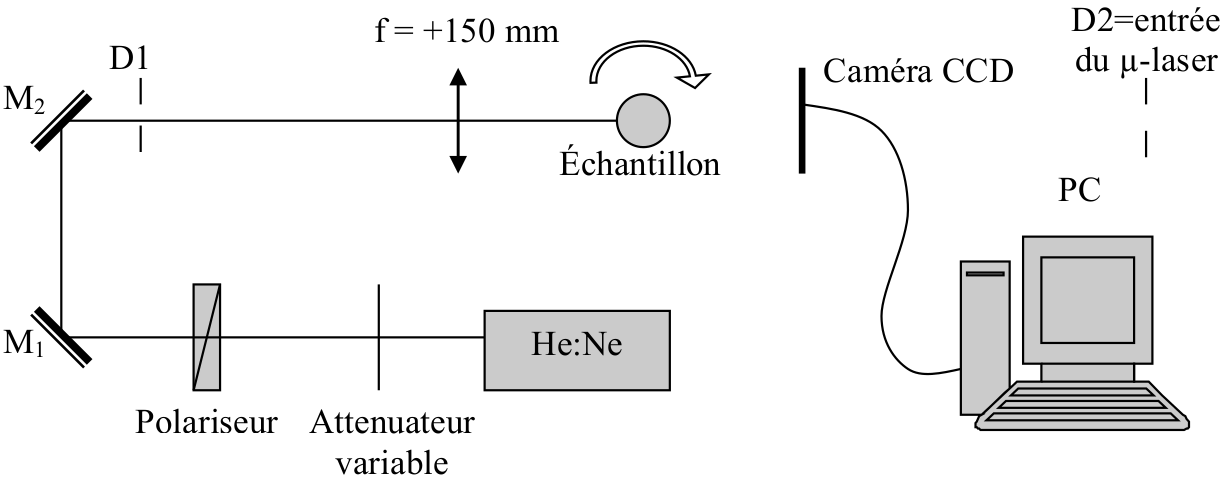
\includegraphics[width=0.7\textwidth]{Images/Schema_exp1}
        \caption{Schéma de l'expérience}
        \label{schema_exp1}
    \end{center}
\end{figure}

On règle l'atténuateur pour avoir, au niveau du capteur CCD, un signal non saturé mais propre.

Le polariseur permet d'éteindre un des spots. En effet on peut polariser intégralement la lumière verticalement ou horizontalement, et dans ce cas seul le spot concerné sera allumé. Ceci permet de vérifier l'orientation du cristal.

On met en place le cristal après une lentille qui permet de refocaliser le faisceau.

Le capteur CCD 1D est placé le plus loin possible du cristal, afin d'obtenir la meilleure précision possible. Néanmoins, plus il est loin, et plus les spots seront défocalisés, et la mesure de la position des spots deviendra difficile. Il est donc nécessaire de faire un compromis.

\section{Orientation du repère optique}
Le cristal est cylindrique, de révolution autour de l'axe optique X. Il s'agit alors de déterminer la direction des axes Y et Z.

Avec les deux spots allumés, on fait tourner le cristal jusqu'à ce qu'ils soient confondus. La direction de propagation est alors soit Y soit Z.

Ensuite, en faisant tourner le cristal, on aura un spot qui ne bougera pas (la polarisation associée à la nappe d'indices circulaire), tandis que l'autre sera dévié (la polarisation associée à la nappe ellipsoïdale).

Si la direction originelle de propagation est Y, ce spot "suivra" la rotation du cristal, tandis qu'il sera dévié dans le même sens si la direction est Z.

\section{Mesure de l'angle entre les spots de polarisation}
On peut retrouver facilement l'angle $\rho$ grâce à la distance entre le capteur et le cristal et la distance entre les deux spots sur le capteur: 
\[  \rho = \frac{d}{2(D(n^+(\theta)-1)-r)} \]
avec:
\begin{itemize}
    \item $d$: la distance entre les spots
    \item $D$: la distance entre le cylindre et le capteur
    \item $r$: le rayon du cylindre
\end{itemize}
\vspace*{0.5cm}
On peut alors tracer l'angle $\rho$ entre les deux spots en fonction de l'angle de rotation du cylindre, ainsi que la courbe théorique associée, sur la figure \ref{courbe1}:

\begin{figure}[h]
    \begin{center}
        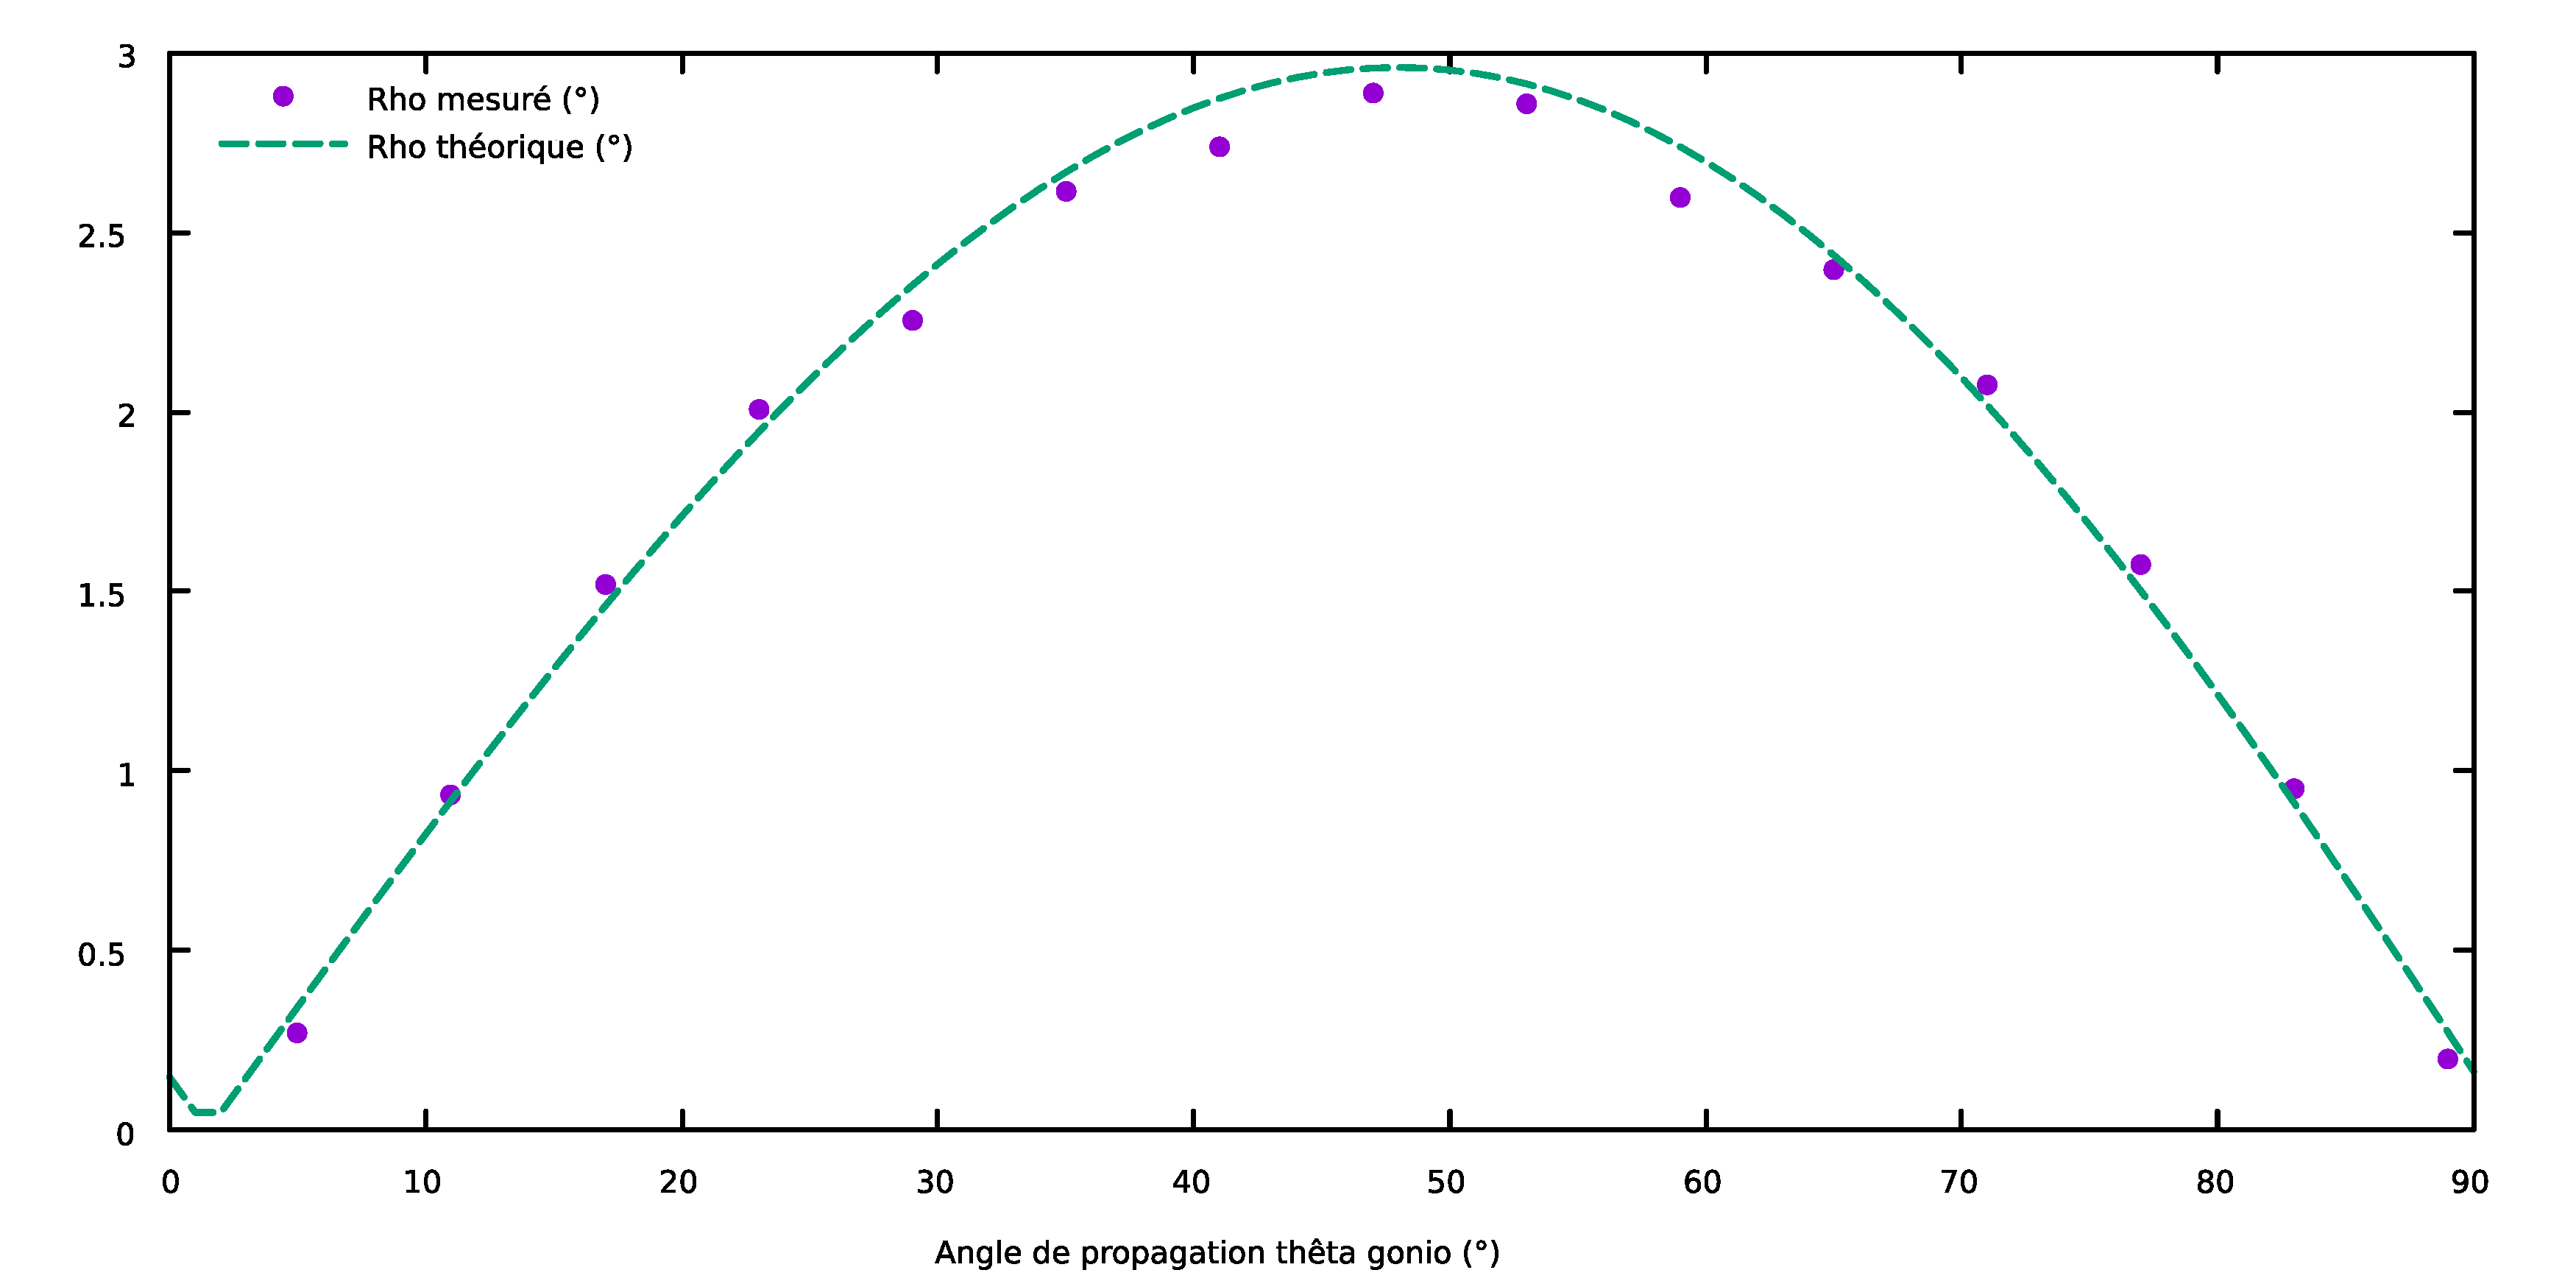
\includegraphics[width=0.8\textwidth]{Images/courbe1}
        \caption{Angle de double réfraction en fonction en fonction de l'angle de propagation $\theta$}
        \label{courbe1}
    \end{center}
\end{figure}

Les résultats expérimentaux sont assez proches de la théorie, à un décalage près en $\theta$ ($\theta_0 = 1,5^o$): le repérage de l'axe optique principal Z est assez précis, mais il aurait pu l'être plus.

\section{Forme des spots}
L'observation de la distance entre les spots nous permet aussi de remarquer leur forme, tracée figure \ref{formespots}.
\begin{figure}[h]
    \begin{center}
        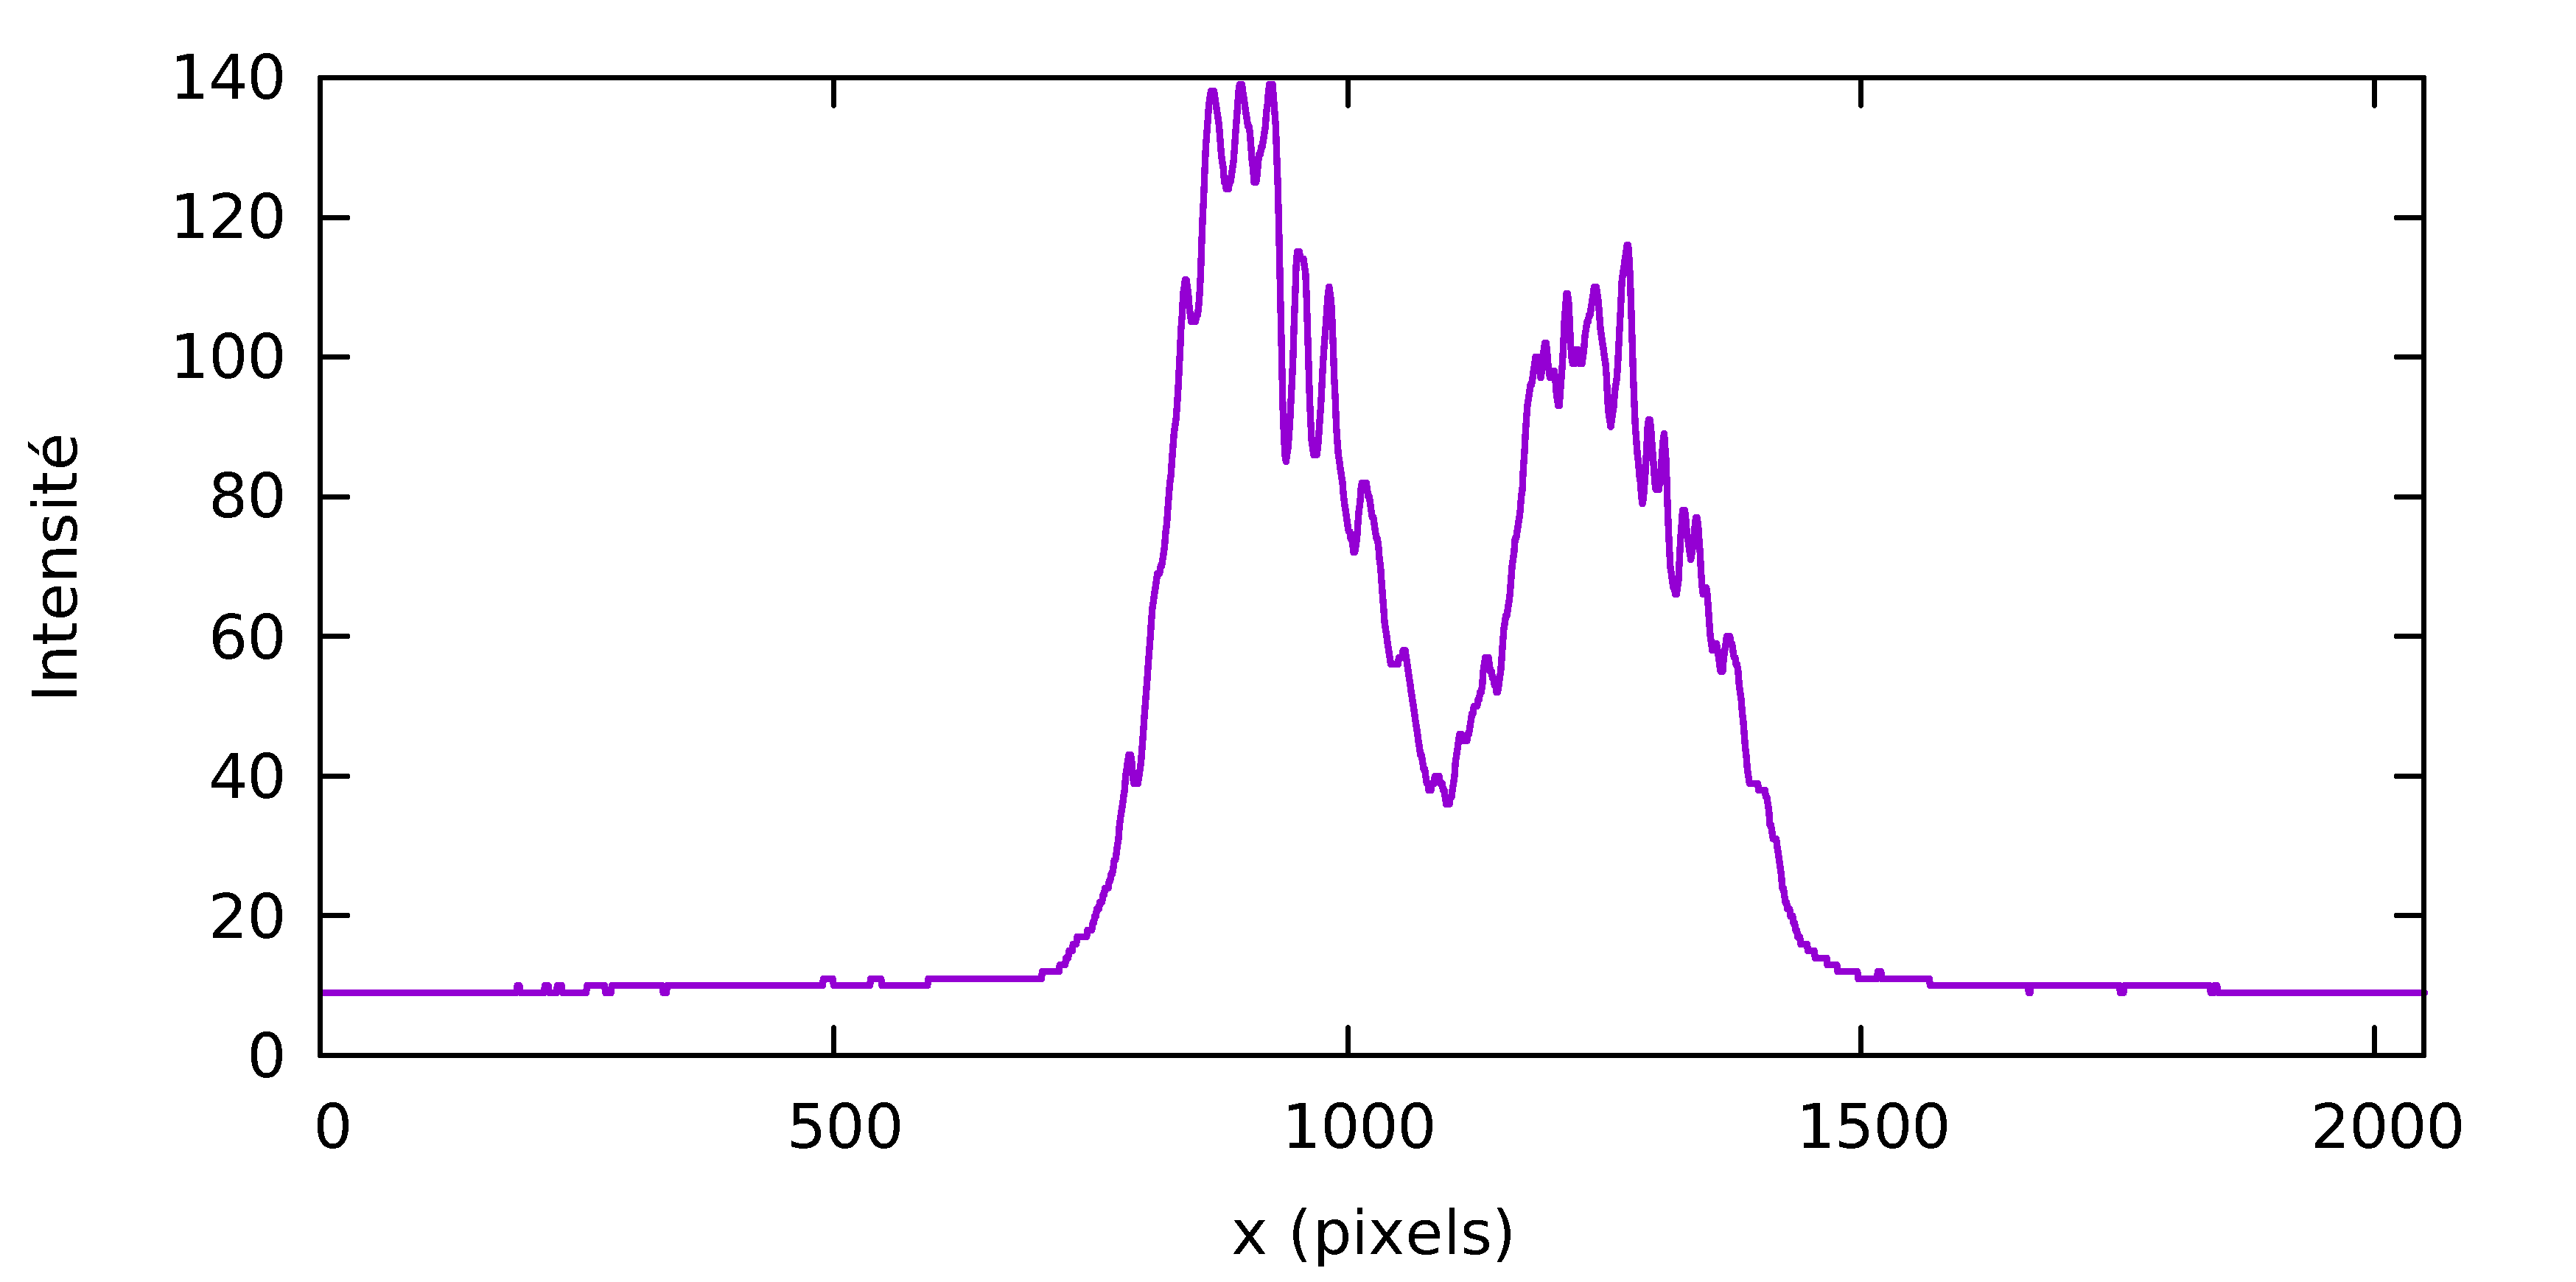
\includegraphics[width=0.8\textwidth]{Images/spots}
        \caption{Intensité reçue par le capteur}
        \label{formespots}
    \end{center}
\end{figure}
On reconnaît un profil de spots gaussiens, nous avons en effet utilisé un laser gaussien.

\chapter{Optique Non-Linéaire: Conversion de fréquences (Théorie)}\label{ONLTheorie}

Maintenant que nous avons vu les effets de l'anisotropie du cristal en réponse linéaire, il nous faut étudier la non-linéarité, notamment la Génération de Seconde Harmonique (SHG). La Génération de Seconde Harmonique est un cas dégénéré de fusion de photons (en considérant l'aspect corpusculaire), elle correspond à l'interaction de deux photons de fréquence $\omega$ qui donnent un photon de fréquence 2$\omega$.

\section{Accord de phase}

L'interaction entre ces 3 photons est maximale si la quantité de mouvement est conservée, on appelle cela la condition d'accord de phase. Cette condition s'écrit :
% $\Delta k$ est le déphasage entre la polarisation non-linéaire et le champ qu'elle génère. La condition d'accord de phase revient à dire:
\[\Delta k=k_3-k_2-k_1=0\]
Avec $\Delta k$ qui est à la fois le déphasage entre la polarisation non-linéaire et le champ qu'elle génère et la différence de quantité de mouvement des photons en intéractions et $k_i$ les normes des vecteurs d'onde mis en jeu lors de l'intéraction.

Or:
\[k_i=\dfrac{2\pi}{\lambda_i}n(\lambda_i)\]

On peut ainsi réécrire $\Delta k$:
\[\Delta k=2\pi\left[\dfrac{n^{\pm}(\lambda_3,\theta,\phi)}{\lambda_3}-\dfrac{n^{\pm}(\lambda_2,\theta,\phi)}{\lambda_2}-\dfrac{n^{\pm}(\lambda_1,\theta,\phi)}{\lambda_1}\right]\]

Il y a ainsi 8 possibilités en fonction du choix de + ou de - pour $n^{\pm}$:

\begin{center}
\begin{tabular}{|c|c|c|}
$\lambda_3$&$\lambda_2$&$\lambda_1$\\
\hline
+&+&+\\
+&+&-\\
+&-&-\\
\hline
-&+&+\\
-&+&-\\
-&-&+\\
\hline
-&-&-\\
\end{tabular}
\end{center}

Les 4 premiers cas sont impossibles car $\lambda_3<\lambda_{1,2}$, or d'après les courbes de $n^+$ et $n^-$, on ne peut avoir $n^+$ avec un longueur d'onde plus faible. Pour des raisons de bijectivité, avoir le même signe partout est impossible. Ce qui laisse 3 possibilités, dont deux dégénérées dans le cas $\lambda_1=\lambda_2$. On notera Type I le cas "-,+,+" et Type II (confondu avec Type III dans notre cas) le cas "-,-,+" (ou "-,+,-").

On remarque ainsi que pour le Type I, on injecte sur les nappes $n^+$, il faudra donc polariser horizontalement, alors que pour le Type II on injecte à la fois sur $n^+$ et $n^-$, il faudra donc un polariseur à 45\textdegree pour injecter simultanément sur ces deux nappes. La polarisation appliquée impose le désaccord de phase, d'où la nécessité d'être capable de contrôler la polarisation (laser polarisé et utilisation systématique de lame $\dfrac{\lambda}{2}$) lors des manipulations.

\section{Condition d'accord de phase dans le cas de l'expérience}

Il nous faut à présent traduire la condition de phase sur des variables modifiables dans le cas de l'expérience. Nous travaillerons dans le plan YZ avec des longueurs d'ondes suivantes:

\indent$\cdot\,\lambda_1=\lambda_2=1,064\mu m=\lambda$\\
\indent$\cdot\,\lambda_3=0,532\mu m=\dfrac{\lambda}{2}$\\

\paragraph{Pour le Type I}
\begin{align*}
\Delta k&=2\pi\left[\dfrac{n^-(\lambda_3,\theta,\phi)}{\lambda_3}-\dfrac{n^+(\lambda_2,\theta,\phi)}{\lambda_2}-\dfrac{n^+(\lambda_1,\theta,\phi)}{\lambda_1}\right]\\
\Delta k&=\dfrac{2\pi\times 2}{\lambda}\left[n^-\left(\dfrac{\lambda}{2},\theta,\dfrac{\pi}{2}\right)-n^+\left(\lambda,\theta,\dfrac{\pi}{2}\right)\right]
\end{align*}

Or: 
\begin{align*}
    &\cdot n^-\left(\dfrac{\lambda}{2},\theta,\dfrac{\pi}{2}\right)=n_x\left(\dfrac{\lambda}{2}\right)\\
    &\cdot n^+\left(\lambda,\theta,\dfrac{\pi}{2}\right)=\dfrac{1}{\sqrt{\dfrac{\cos^2\theta}{n_y^2(\lambda)}+\dfrac{\sin^2\theta}{n_z^2(\lambda)}}}
\end{align*}

Ainsi, après calculs, on obtient: 
\[\sin^2\theta_{I}=\dfrac{\dfrac{1}{n_x^2(\lambda/2)}-\dfrac{1}{n_y^2(\lambda)}}{\dfrac{1}{n_z^2(\lambda)}-\dfrac{1}{n_y^2(\lambda)}}\]

D'où: 
\[\theta_{I}=41^{\circ}\]

\paragraph{Pour le Type II}
\[\Delta k=\dfrac{2\pi}{\lambda}\left[2n^-\left(\dfrac{\lambda}{2},\theta,\dfrac{\pi}{2}\right)-n^-\left(\lambda,\theta,\dfrac{\pi}{2}\right)-n^+\left(\lambda,\theta,\dfrac{\pi}{2}\right)\right]\]

Avec les mêmes expressions pour $n^-(\lambda/2)$ et $n^+(\lambda)$ mais avec:
\[\cdot\,n^-(\lambda)=n_x(\lambda)\]

Ainsi, après calculs, on obtient cette fois:
\[\sin^2\theta_{II}=\dfrac{\dfrac{1}{(2n_x(\lambda/2)-n_x(\lambda))^2}-\dfrac{1}{n_y^2(\lambda)}}{\dfrac{1}{n_z^2(\lambda)}-\dfrac{1}{n_y^2(\lambda)}}\]

D'où:
\[\theta_{II}=76^{\circ}\]

La condition d'accord de phase se traduit donc par un angle $\theta$ imposé. Cependant, l'accord de phase traduit un maximum d'interactions entre les 3 photons. Ainsi, les angles trouvées devraient être des maxima d'intensité de lumière à $2\omega$ et non pas des directions exclusives (même si c'est assez sélectif, comme nous le verrons).

\section{Calculs de $\chi$ (Type I et Type II)}

Nous avons à présent les angles $\theta$ dans lesquelles on devrait voir apparaître la génération de seconde harmonique, donc une lumière de longueur d'onde égale à $0,532\mu m$, pour les Types I et II. Cependant, il reste un point important à vérifier: le  cristal possède-t-il un coefficient de susceptibilité électrique non linéaire non nul pour ces directions ? C'est ce que nous allons vérifier grâce au calcul de $\chi_{eff}$.

\paragraph{Pour le Type I}
On ecrit l'expression de la susceptibilité effective:

\[\chi_{eff}^{SHG_I}=\sum_{i,j,k}e^-_j(\lambda/2)\chi_{j,i,k}(\lambda/2)e^+_i(\lambda)e^+_k(\lambda)\]

Avec {i,j,k}={x,y,z} car $\chi^{(2)}$ est un tenseur de 27 éléments, mais beaucoup sont nuls, pour des raisons de symétrie du cristal. On se réfère alors à des tables de $\chi^{(2)}$ qui nous fournissent les éléments non nuls, notamment pour le groupe de symétrie 2mm auquel le RTP appartient. Mais avant de regarder cette table, on réduit d'abord les possibilités avec le produit vectoriel des polarisations: $e^-_j(\lambda/2)e^+_i(\lambda)e^+_k(\lambda)$.

En effet, on note:
\[f_{j,i,k}=\begin{pmatrix}-1\\0\\0\end{pmatrix}\begin{pmatrix}0\\-\cos\theta'\\\sin\theta'\end{pmatrix}\begin{pmatrix}0\\-\cos\theta'\\\sin\theta'\end{pmatrix}\]

Les coefficients $f_{j,i,k}$ sont presque tous nuls sauf $f_{x,y,y}$, $f_{x,z,z}$, $f_{x,y,z}$ et $f_{x,z,y}$. 
On peut à présent comparer avec les coefficients non nuls de $\chi^{(2)}$. Or, d'après la table, les quatre coefficients correspondants sont nuls.

Cela implique:
\[\chi_{eff}^{SHG_I}=0\]

Ainsi, la symétrie du cristal de RTP empêche la génération de seconde harmonique en polarisant la lumière selon les nappes $n^+$. On ne verra donc aucune lumière à $0,532\mu m$ en polarisant horizontalement uniquement. Il reste à réaliser la même étude pour le Type II.

\paragraph{Pour le Type II}

On reprend la même étude avec l'expression: 

\[\chi_{eff}^{SHG_I}=\sum_{i,j,k}\chi_{j,i,k}(\lambda/2)e^-_j(\lambda/2)e^+_i(\lambda)e^-_k(\lambda)\]

Dans ce cas:

\[f_{j,i,k}=\begin{pmatrix}-1\\0\\0\end{pmatrix}\begin{pmatrix}0\\-\cos\theta'\\\sin\theta'\end{pmatrix}\begin{pmatrix}-1\\0\\0\end{pmatrix}\]

Alors, $f_{x,y,x}$ et $f_{x,z,x}$ sont non nuls, et d'après les tables $\chi_{x,y,x}$ est nul mais $\chi_{x,z,x}$ ne l'est pas. 

Comme $f_{x,z,x}=\sin\theta'$, on peut écrire:

\[\chi_{eff}^2=\chi_{x,z,x}^2\sin^2\theta'\neq 0\]

On peut donc avoir de la génération de seconde harmonique de Type II sur le cristal de RTP. Cependant, on remarque que $\chi_{eff}$ est maximal pour $\theta'\simeq\theta=90$\textdegree, or la condition d'accord de phase nous impose $\theta=76$\textdegree. Le rendement ne sera donc pas idéal, pour s'en approcher, il faudrait changer les longueurs d'ondes en jeu pour modifier l'angle imposé par la condition d'accord de phase (cf courbe d'accord de phase). Cependant, il est impossible d'avoir 0\% de rendement d'après ces mêmes courbes car $\theta=0$ n'est jamais solution de la condition d'accord de phase.

Il nous faut alors mettre en place l'expérience de SHG Type II afin de valider ces calculs, notamment vérifier l'angle trouvé.

\chapter{Optique Non-Linéaire: Conversion de fréquences (Expérience)} \label{ONLExp}
Après avoir établi certains paramètres pour l'expérience, il faut la mettre en place afin de les vérifier.
\section{Mise en place de l'expérience pour une SHG de type II}
Le montage ressemblera à celui vu précédemment, avec des miroirs pour calibrer le faisceau comme on le souhaite (Fig \ref{montageONL}), cependant, on utilise cette fois un laser à $1,064\mu m$ soit invisible pour l'oeil humain et très puissant. Les consignes de sécurité sont alors bien plus strictes à cause de la dangerosité de ce laser. On met des lunettes de protections (pour la longueur d'onde considérée) et on ne place jamais nos yeux à hauteur du banc d'optique. On fait également attention à prévenir lorsqu'on allume le laser, comme on ne le voit pas. On peut vérifier la présence du faisceau grâce à un des cristaux qui emmettent du rouge lorsqu'ils reçoivent de l'infrarouge (placés sur une petite plaquette).

\begin{figure}
\centering
    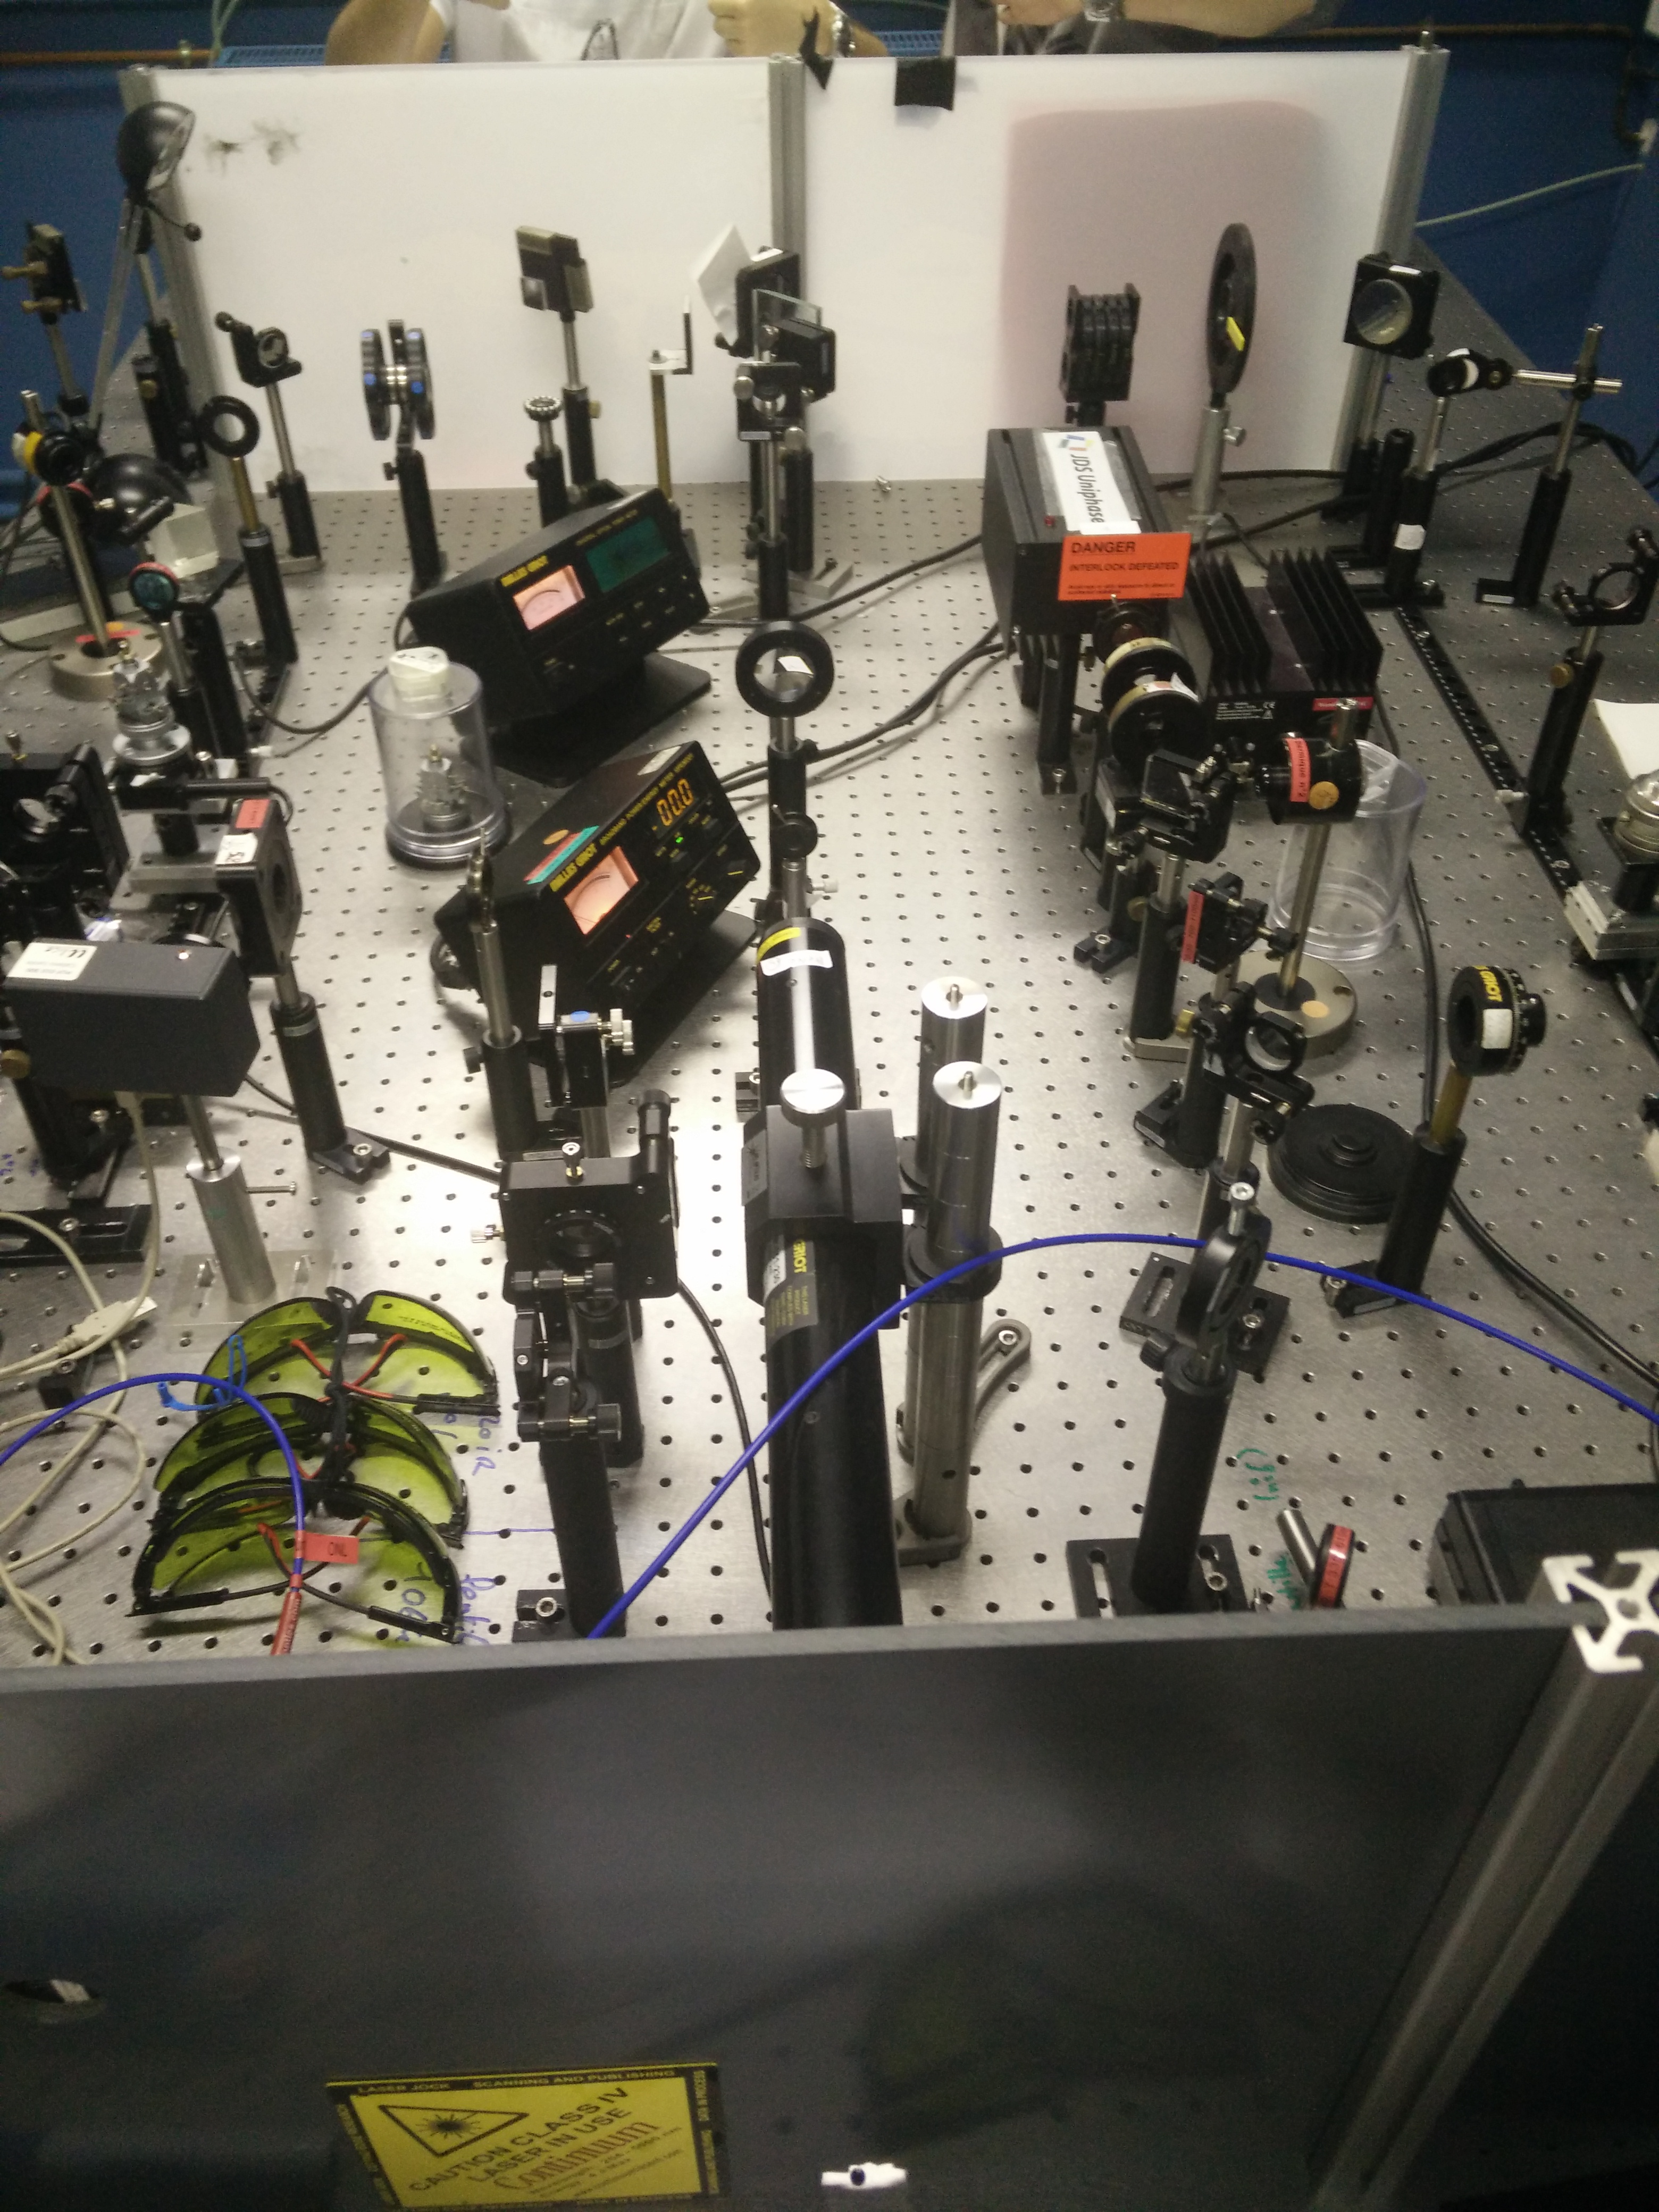
\includegraphics[width=200pt]{Photos/montage2}
    \caption{Photo du montage pour la SHG}
    \label{montageONL}
\end{figure}
\section{Mesure des angles d'accord de phase}
On observe le faisceau en sortie du cristal, avec un écran blanc. On fait tourner le cristal afin de se placer dans les directions $\theta$ trouvées précédemment, sans connaître le repère. Donc on tourne juste jusqu'à faire apparaître un faisceau vert. Une fois une des directions trouvées, on essaye de repérer à l'oeil le maximum d'intensité, puis on note le repère angulaire du goniomètre. On fait ensuite tourner le cristal pour repérer les 3 autres angles (cristal biaxe: donc deux axes symétriques, on place ensuite ces repères sur un cercle, car on ne connait pas le repère optique, donc on ne peut déterminer directement $\theta_{II}$.

Nous avons trouvé des directions de maxima aux repères 30, 58, 210 et 238 degrés du goniomètre (Voir Fig. \ref{anglesONL}. On trouve alors $\theta=\dfrac{210-58}{2}=\dfrac{390-238}{2}=76$\textdegree, ce qui vérifie bien la valeur trouvée précédemment grâce à la théorie.

\begin{figure}
    \centering
    \begin{tikzpicture}[scale=1.5]
    \draw [->](-3,0)--(3,0);
    \draw (3,0)node[below]{$Y$};
    \draw [->](0,-3)--(0,3);
    \draw (0,3)node[left]{$Z$};
    \draw (2,0) arc(0:14:2) --(0,0);
    \draw (-2,0) arc(180:180-14:2)--(0,0);
    
    \draw (2,0) arc(0:-14:2) --(0,0);
    \draw (-2,0) arc(180:180+14:2)--(0,0);
    \draw [thick] (0,0) circle(2);
    \draw [dotted] (2,0) arc (0:-44:2)--(0,0) node[midway, below]{\small "0" du goniomètre};
    \end{tikzpicture}
    \caption{Vue de dessus du cristal et des directions des maxima d'intensité du faisceau vert}
    \label{anglesONL}

\end{figure}

\section{Mesure de la longueur d'onde générée}
Cependant, il reste à vérifier que l'on génère bien la longueur d'onde moitié (et pas deux longueurs d'ondes proches par exemple). On utilise alors un spectromètre pour trouver la longueur d'onde du faisceau vert (Fig \ref{spectro}). On remarque qu'il n'y a que deux pics, l'incident à $1,064\mu m$ et la longueur d'onde moitié $0,532\mu m$, on a donc bien une génération de seconde harmonique.

\begin{figure}[H]
\centering
    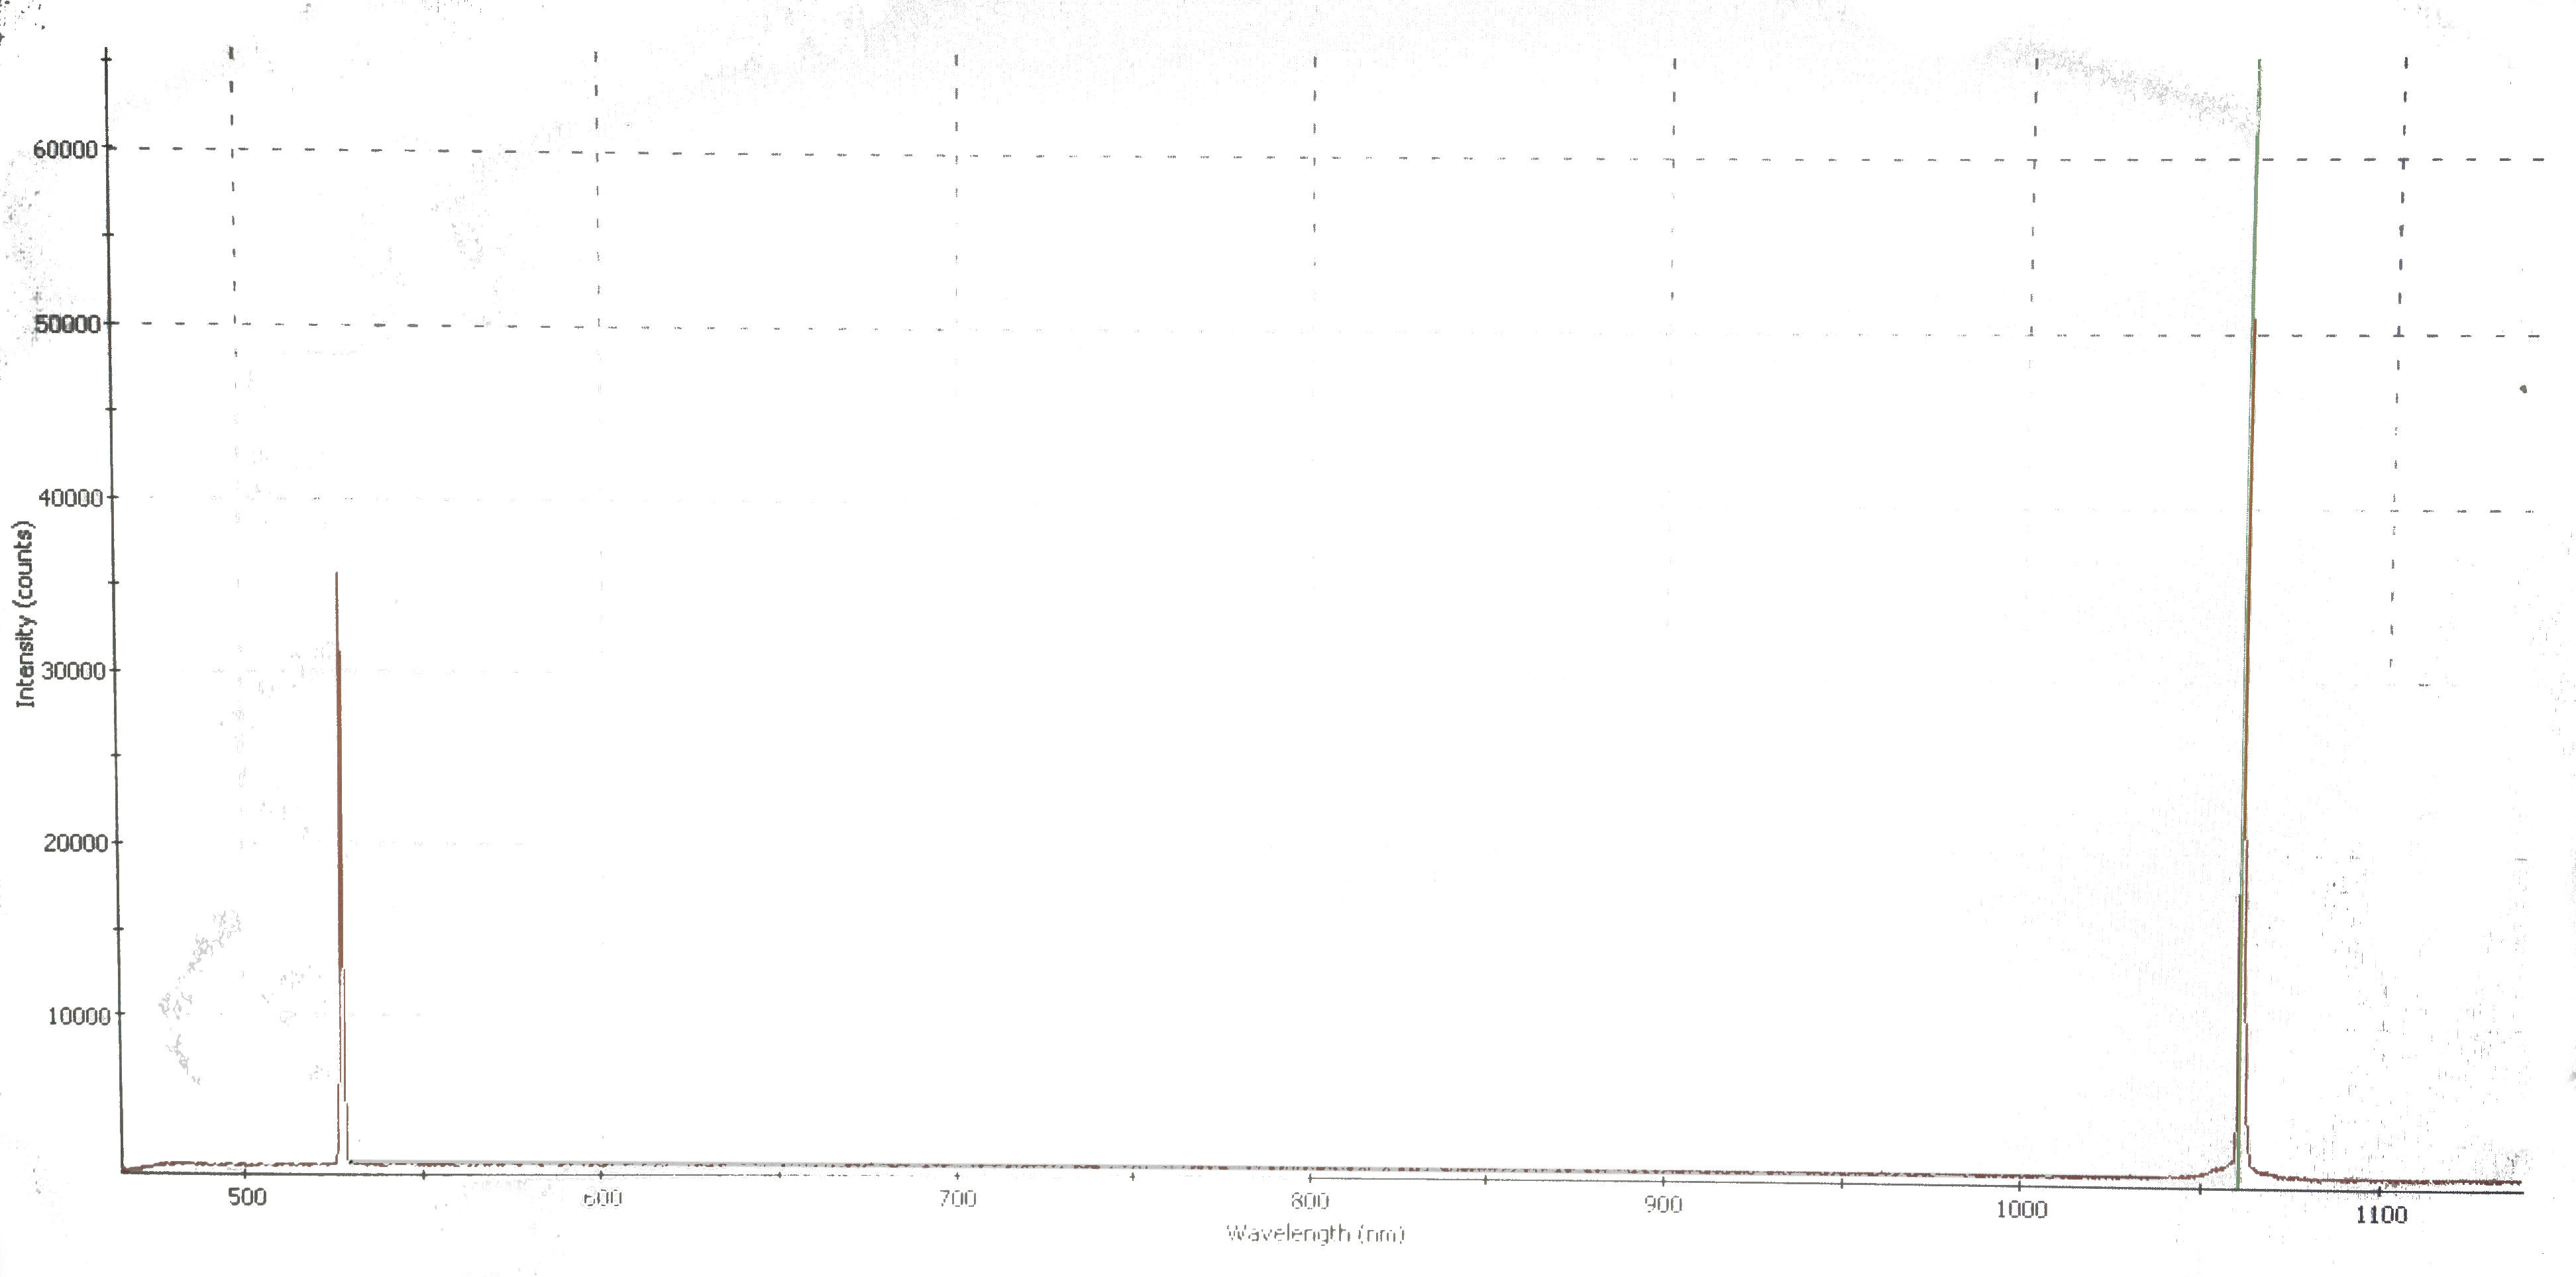
\includegraphics[width=300pt]{Photos/courbe}
    \caption{Spectrogramme après le cristal}
    \label{spectro}
\end{figure}

\section{Vérification de la loi quadratique}
On cherche ensuite à déterminer comment varie l'intensité de la lumière à $\lambda/2$ par rapport à l'intensité incidente. On mesure la puissance incidente et la puissance après le cristal en séparant les longueurs d'ondes grâce à un prisme. L'intensité de la longueur d'onde générée est censée varier quadratiquement en fonction de l'intensité incidente. En Figure \ref{Intesité}, nous avons tracé les intensités mesurées (en soustrayant l'offset du à la luminosité de la salle (150nW), car même en travaillant dans le noir, il reste de la lumière parasite), cependant on ne retrouve pas de relation quadratique, on remarque au contraire que la courbe est plutôt linéaire. Multiplier l'intensité par deux ne multiplie pas l'intensité verte par 4. 

\begin{figure}[H]
    \centering
    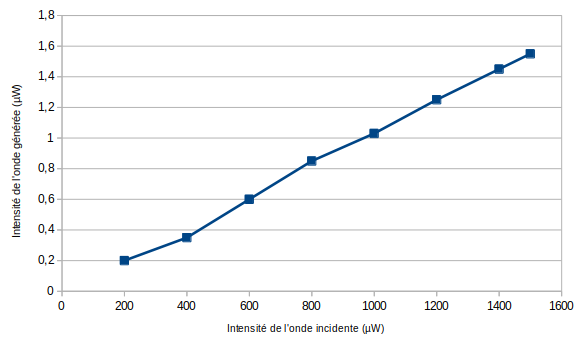
\includegraphics[width=250pt]{Photos/graphe}
    \caption{Intensité de l'onde générée en fonction de l'intensité de l'onde incidente}
    \label{Intensité}
\end{figure}


\chapter*{Conclusion} \addcontentsline{toc}{chapter}{Conclusion}
Au cours de ce TP nous avons pu mettre en évidence les concepts décrits théoriquement en cours. Nous avons pu observer grâce au laser et à sa forme cylindrique spécifique, l'anisotropie du cristal de RTP qui sépare les différentes polarisations de la lumière, mais également les effets non-linéaires qui peuvent intervenir sous certaines conditions. Nous avons réalisé ces expériences en accord avec la théorie, en vérifiant celle-ci grâce aux expérimentations. Ces effets non linéaires sont important pour certaines applications, notamment par exemple la génération de laser aux fréquences TeraHertz, car technologiquement c'est difficile à produire mais avec des sommes ou des soustractions de fréquence de laser existant, cela devient possible.


\end{document}
